\documentclass[../main.tex]{subfiles}
\begin{document}
    \chapter{Research Method}\label{chap:research_method}

    %This section will contain:
    %TODO: Explain the used method. %TODO research method
    %TODO: Hypothese/research questions %TODO research question

    \section{Introduction}
    $<<$ Todo: properly introduction of this chapter $>>$
    \\
    The type inference analysis will be performed in this order:
    \begin{itemize}
        \item Resolve types
        \item Resolve sub type relations
        \item Extract facts from the source code
        \item Extract constraints from source code
        \item Solve the constraints
    \end{itemize}
    In the next step, annotations will be added to see how the results be like.
    
    \section{Research Question}
    The research question will be something like: \\
    \begin{quote}
        Will the use of phpdoc annotations produce better (to be defined) results for constraint based type inference?
    \end{quote}

    \begin{quotation}
    quotation
    \end{quotation}



    \section{Types}
    Explain here what I mean with a type...
    
    \begin{rascal}
\CAT{Keyword}{module} lang::php::m3::TypeSymbol

\CAT{Keyword}{data} TypeSymbol
  = any()
  | array(\CAT{Keyword}{TypeSymbol} arrayType)
%  | array()
  | \textbackslash{}bool()
  | class(\CAT{Keyword}{loc} decl)
  | float()
  | \textbackslash{}int()
  | object()
  | resource()
  | \textbackslash{}null()
  | string()
  | unset()
  ; 
    \end{rascal}
    
    \subsection{PHP types}
    PHP has a similar class inheritance structure and interface implementation as Java.
    The main difference is that in PHP all class are \texttt{public} and that inner classes are not allowed in PHP. 
    \\
    The basis types in PHP are integers, floats (similar to doubles and reals), booleans, strings, arrays, resources and null.
    When variables are initialised without a values, they are null. The recourse type is a special one which is not important for this research.
 
    \subsection{Subtypes}
    
    Explain something about subtypes here. For now, only this figure\ref{fig:subtypeTree}

    \begin{figure}[H]
        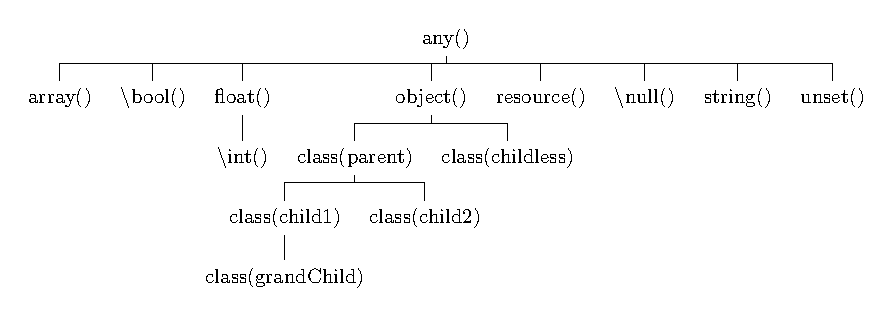
\includegraphics{Diagrams/Subtypes.pdf}
        \caption{Subtype hierarchy}
        \label{fig:subtypeTree}
    \end{figure}

    The subtype relation of class inheritance is a \gls{reflexive transitive closure} relation.
    A class extension of \textbf{\texttt{class A}} on \textbf{\texttt{class C}} will define \textbf{\texttt{class A}} as a subtype of \textbf{\texttt{class C}} in our analysis, as you can see in figure \ref{fig:subtypes}.
    If a class does not extend another class, it will implicitly extend the \gls{stdClass} class.
    You can see that this happens with \textbf{\texttt{class D}} in the example.
    The \textbf{\texttt{stdClass}} is represented as the type \textbf{\texttt{object()}} in our analysis.
    \\
    The basic PHP types also contain a subtype relation.
    Integers are subtypes of floats.
 
    % show three images next to each other
    \begin{figure}[H]
    \begin{subfigure}[b]{.33\textwidth}
      \begin{center}
      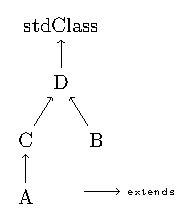
\includegraphics[scale=1]{Diagrams/Inheritance_example.pdf}
      \caption{Inheritance relation}
      \label{fig:subtype}
      \end{center}
    \end{subfigure}
    \begin{subfigure}[b]{.33\textwidth}
      \begin{center}
      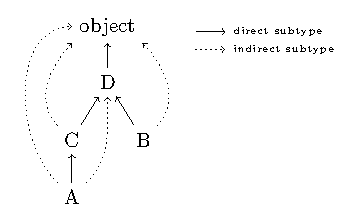
\includegraphics[scale=1]{Diagrams/Subtypes_example.pdf}
      \caption{Subtype relation}
      \label{subtype_tc}
      \end{center}
    \end{subfigure}
    \begin{subfigure}[b]{.33\textwidth}
      \begin{center}
      \lstinputlisting[xleftmargin=20pt,xrightmargin=20pt,language=PHP]{src/php/inheritance.php}
      \caption{Inheritance in PHP}
      \label{subtype_code}
      \end{center}
    \end{subfigure}
    \caption{Relation of subtypes among classes}
    \label{fig:subtypes}
    \end{figure}
    
    \section{Fact extraction}
    We can extract fact about classes, class-constants/fields/methods, functions, parameters.
    For these facts, we can use a relation, so we have a many-to-many relation.
    On the left size we will have the class, function or method. On the right side we have their attribute.
    \\
    A list of properties: (todo: rewrite this list into a `normal' section.) %todo rewrite this piece
    \begin{itemize}
        \item \textless{}loc classDecl, className(str name)\textgreater{}
        \item \textless{}loc classDecl, classMethod(str name, set[Modifier] modifiers)\textgreater{}
        \item \textless{}loc classDecl, classProperty(str name, set[Modifier] modifiers)\textgreater{}
        \item \textless{}loc classDecl, classConstant(str name, set[Modifier] modifiers)\textgreater{}
        \item \textless{}loc classDecl, classConstructorParameters(list[PhpParam] params)\textgreater{}
        
        \item \textless{}loc methodDecl, methodName(str name)\textgreater{}
        \item \textless{}loc methodDecl, methodParameters(list[PhpParam] params)\textgreater{}
        %\item \textless{}loc methodDecl, methodHasReturnStatements(bool)\textgreater{}
        
        \item \textless{}loc functionDecl, functionName(str name)\textgreater{}
        \item \textless{}loc functionDecl, functionParameters(list[PhpParam] params)\textgreater{}
    \end{itemize}
    
    In Rascal:
    \begin{rascal}
\CAT{Keyword}{alias} TypeFacts = \CAT{Keyword}{rel}{}[\CAT{Keyword}{loc} decl, Fact fact];

\CAT{Keyword}{data} Fact
    = className(\CAT{Keyword}{str} name) \CAT{Comment}{// = FQN = fully qualified name}
    | classMethod(\CAT{Keyword}{str} name)
    | classProperty(\CAT{Keyword}{str} name)
    | classConstant(\CAT{Keyword}{str} name)
    | classConstructorParameters(\CAT{Keyword}{list}{}[PhpParam] params)
    | methodName(\CAT{Keyword}{str} name)
    | methodParameters(\CAT{Keyword}{list}{}[PhpParam] params)
    | functionName(\CAT{Keyword}{str} name)
    | functionParameters(\CAT{Keyword}{list}{}[PhpParam] params)
    ;
    \end{rascal}

    Other facts that will be used:
    \begin{rascal} 
\CAT{Keyword}{alias} PhpParams = \CAT{Keyword}{lrel}{}[\CAT{Keyword}{loc} decl, \CAT{Keyword}{set}{}[\CAT{Keyword}{loc}] typeHints, \CAT{Keyword}{bool} isRequired, \CAT{Keyword}{bool} byRef];
\CAT{Keyword}{data} Annotation = returnType(\CAT{Keyword}{set}{}[TypeSymbol]) | parameterType(\CAT{Keyword}{loc} var, \CAT{Keyword}{set}{}[TypeSymbol])
    | varType(\CAT{Keyword}{loc} var, \CAT{Keyword}{set}{}[TypeSymbol]);

\CAT{Keyword}{anno} \CAT{Keyword}{rel}{}[\CAT{Keyword}{loc} from, \CAT{Keyword}{loc} to] M3@containment;          \CAT{Comment}{// 'from' directly contains 'to'}
\CAT{Keyword}{anno} \CAT{Keyword}{rel}{}[\CAT{Keyword}{loc} from, \CAT{Keyword}{loc} to] M3@extends;              \CAT{Comment}{// 'from' extends 'to' }
\CAT{Keyword}{anno} \CAT{Keyword}{rel}{}[\CAT{Keyword}{loc} from, \CAT{Keyword}{loc} to] M3@implements;           \CAT{Comment}{// 'from' implements 'to' }
\CAT{Keyword}{anno} \CAT{Keyword}{rel}{}[\CAT{Keyword}{loc} decl, PhpParams params] M3@parameters; \CAT{Comment}{// formal parameters of functions/methods}
\CAT{Keyword}{anno} \CAT{Keyword}{rel}{}[\CAT{Keyword}{loc} decl, \CAT{Keyword}{loc} to] M3@constructors;         \CAT{Comment}{// 'decl' and its constructor 'to'}
\CAT{Keyword}{anno} \CAT{Keyword}{rel}{}[\CAT{Keyword}{loc} decl, Annotation annotation] M3@annotations;  \CAT{Comment}{// result of parsed php docs}

    \end{rascal}
    
    \subsection{Type extraction}
    In order to define the subtype relations in class extensions, we will need to declare all existing class types.
    We can do this in rascal like is done in the example below:
    \begin{rascal}
\CAT{Keyword}{visit} (system) \{{}
    \CAT{Keyword}{case} c:class(\_{}, \_{}, \_{}, \_{}, \_{}): types += class(c@decl);
\}{}
    \end{rascal}
    Once all types are defined, we can add the subtype relation. We will need to have the subtype of \texttt{int()} and \texttt{float()} and the class extensions.
    You can see that in the code below:
    \begin{rascal}
\CAT{Keyword}{public} \CAT{Keyword}{rel}{}[TypeSymbol, TypeSymbol] getSubTypes(M3 m3, System system) 
\{{}
    \CAT{Keyword}{rel}{}[TypeSymbol, TypeSymbol] subtypes
        \CAT{Comment}{// add int() as subtype of float()}
        = \{{} \textless{}\textbackslash{}int(), float()\textgreater{} \}{} 
        \CAT{Comment}{// use the extends relation from M3}
        + \{{} \textless{}class(c), class(e)\textgreater{} | \textless{}c,e\textgreater{} \textless{}- m3@extends \}{}
        \CAT{Comment}{// add subtype of object for all classes which do not extends a class}
        + \{{} \textless{}class(c@decl), object()\textgreater{} | l \textless{}- system, /c:class(n,\_{},noName(),\_{},\_{}) \textless{}- system{}[l] \}{};
        
    \CAT{Comment}{// compute reflexive transitive closure and return the result }
    \CAT{Keyword}{return} subtypes*;        
\}{}
    \end{rascal}
  
    \subsection{Constraint extraction}
       
    Introduction is needed here... for now I will just list the types that I have found.
    Maybe this needs to be moved to a different chapter.
    \\
    \textbf{This is a list of items which are not supported (yet)}:

    \begin{itemize}
        
        \item References (in PHP they are symbol table aliases)
        \begin{itemize}
            \item on expression assignments :: $\$a \; = \; \&\$b$
            \item on functions :: function $\&f()$ $\{ \dots \}$
            \item on parameters :: function $f(\&\$a)$ $\{ \dots \}$             
        \end{itemize}

        \item Variable structures:
        \begin{itemize}
            \item \sout{Variable variables} :: $\$\$a;$
            \item \sout{Variable class instantiation} :: $new \; \$a;$
            \item \sout{Variable method or function calls} :: $\$a();$
        \end{itemize}

        \item List assign :: $list(\$a, \$b) = array("one", "two");$ (we can assume that the rhs is of type array, when the program is correct)
        
        \item \sout{Method or function parameters (including type hints)}
        \item \sout{Class structures, method calls}
        \item Class Constants
        
        \item \sout{The global statement} (should be resolved by the usage relation from M3)
        
        \item \sout{Casts of expressions}
        
        \item \sout{Predefined variables} (\$this, self, parent, static)

        \item \sout{Eval} (will not be supported)        
        \item \sout{Closures} (not used much in production code)
        \item \sout{Traits} (not used much in production code)
        \item \sout{Callable} (introduced in 5.4 as typehint, not used much in production code)
        
        \item Foreach(\$a as ... (=> ...)) => \$a is an array or an object;
        \item \sout{return; => return type is null} (is added to the situation when there are no return statements)
        \item add predefined globals (and their type: \$[GLOBALS, \_SERVER, \_GET, \_POST, \_REQUEST, \_COOKIE, \_ENV, \_SESSION, php\_errormsg] (all in global scope))
        \item add magic constants: \_\_[DIR, FILE, LINE, NAMESPACE, FUNCTION, CLASS, METHOD]\_\_
        \item predefined constants: TRUE(b), FALSE(b), NAN(f), INF(f), NULL(n), STDIN(r), STDOUT(r), STDERR(r) 
        \item define("name", value) mixed with constants (?out of scope?)
        \item \sout{keywords: self, parent, static in a class} (is included in method and property calls        
    \end{itemize}

    \hrulefill
    
    \textbf{Legend} \\
    \begin{table}[H]
        \begin{tabular}{ c c l c c l }
            $=$     & = & Equal to (type) &
            $C$     & = & A class \\
            $<:$    & = & Is subTypeOf &
            $\rightarrow c$     & = & A class constant \\
            $E_k$   & = & An expression &
            $\rightarrow p$     & = & A class property \\
            $[E_k]$ & = & Type of some expression &
            $\rightarrow m$     & = & A class method \\
            $f$     & = & A function &
            $[m]$   & = & (Return) type of a method call \\
            $[f]$   & = & (Return) type of a function &
            $(A_n)$ & = & The n'th actual argument \\
            $::c$   & = & Static property fetch &
            $(P_n)$ & = & The n'th formal parameter \\
            $::m$   & = & Static method call &
            $th$    & = & Type hint \\
            $::p$   & = & Static property fetch &
            $v$     & = & Default value \\
            Mfs     & = & Modifiers &
            $\Gamma$ & = & Whole program 
            
            
        \end{tabular}
        \caption{Constraint legend}
        \label{table:constraintLegend}
    \end{table}
    
    \subsubsection{Expressions}
    \fact{assignment1}{Normal assignment}{}
    \fact{ternary}{Ternary}{}
    \fact{assignment2}{Assignments with operators (1)}{always resulting in ints}
    \fact{assignment3}{Assignments with operators (2)}{string concat ($.=$)}
    \fact{assignment4}{Assignments with operators (3)}{resulting in int where rhs is no array}
    \fact{assignment5}{Assignments with operators (4)}{resulting in int or float}
    \fact{unaryOperators}{Unary operators}{}
    \fact{binaryOperators}{Binary operators}{}
    \fact{comparisonOperators}{Comparison operators}{}
    
    \subsubsection{Array}
    \fact{arrayAccess}{Array value fetch}{}
    \fact{array}{Array declaration}{}

    \subsubsection{Scalars}
    \fact{scalar}{Scalars}{}
    \fact{encapsed}{Encapsulated strings}{}
    
    \subsubsection{Casts}
    \fact{casts}{Casts}{\\ {\footnotesize{Note: PHP Warnings are ignored}}}
            
    \subsubsection{Clone}
    \fact{clone}{Clone}{}
    
    \subsubsection{Class}
    \fact{instantiation1}{Class instantiation (1)}{matching the class name}
    \fact{instantiation2}{Class instantiation (2)}{of an expression}
    \fact{keywords}{Special keywords}{\texttt{self}\, \texttt{parent} \texttt{parent} \texttt{static}}
    \fact{property1}{Class property fetch}
        {\\ \footnotesize{* Possible add fact that the field E is declared in class C, when it is on the left side of an assignment.}}
    \fact{property2}{Class property fetch variable}{}
    \fact{methodCall1}{Class method call}{}
    \fact{methodCall2}{Class method call variable}{}
    \fact{classConstants}{Class constants (needs to be reviewed)}{}
    
    \subsubsection{Parameters}
    \fact{parameter1}{Parameters in class instantiation}{
        \\
        \footnotesize{*These parameters are just examples for what happens if they have typeHints ($th$), default values($v$) or none}
        \footnotesize{*The constructor can be found in the m3 model (@constructors(loc classDecl, loc constructorMethodDecl))}
    }
    \fact{function1}{Type of a certain variable within some scope}{\\ {\footnotesize{this applies to global- class- function- and method- scope}}}
    \fact{return1}{Return type of function or method (1)}{having no return statements or \texttt{return;}}
    \fact{return2}{Return type of function or method (2)}{every exit path ends with a return statement}
    \fact{return3}{Return type of function or method (3)}{possible no return value}
    \fact{functionCall1}{Function call}{}
    \fact{functionCall2}{Function call variable}{}
    
    How to resolve expressions:
    \begin{itemize}
        \item Find all expressions which are defined above and annotate them with @type.
        \item Annotate the rest of the expressions with @type = any(); (should only be for relevant expressions)
    \end{itemize}
    
    \section{Annotations}
    Explain how the annotations are added to the constraints.
    
    \section{Constraint solving}
    Explain how we will solve constraints.


\end{document}
